\documentclass{extbook}[14pt]
\usepackage{multicol, enumerate, enumitem, hyperref, color, soul, setspace, parskip, fancyhdr, amssymb, amsthm, amsmath, latexsym, units, mathtools}
\everymath{\displaystyle}
\usepackage[headsep=0.5cm,headheight=0cm, left=1 in,right= 1 in,top= 1 in,bottom= 1 in]{geometry}
\usepackage{dashrule}  % Package to use the command below to create lines between items
\newcommand{\litem}[1]{\item #1

\rule{\textwidth}{0.4pt}}
\pagestyle{fancy}
\lhead{}
\chead{Answer Key for Makeup Progress Quiz 3 Version A}
\rhead{}
\lfoot{1648-1753}
\cfoot{}
\rfoot{Summer C 2021}
\begin{document}
\textbf{This key should allow you to understand why you choose the option you did (beyond just getting a question right or wrong). \href{https://xronos.clas.ufl.edu/mac1105spring2020/courseDescriptionAndMisc/Exams/LearningFromResults}{More instructions on how to use this key can be found here}.}

\textbf{If you have a suggestion to make the keys better, \href{https://forms.gle/CZkbZmPbC9XALEE88}{please fill out the short survey here}.}

\textit{Note: This key is auto-generated and may contain issues and/or errors. The keys are reviewed after each exam to ensure grading is done accurately. If there are issues (like duplicate options), they are noted in the offline gradebook. The keys are a work-in-progress to give students as many resources to improve as possible.}

\rule{\textwidth}{0.4pt}

\begin{enumerate}\litem{
Determine the domain of the function below.
\[ f(x) = \frac{4}{15x^{2} -5 x -20} \]The solution is \( \text{All Real numbers except } x = -1.000 \text{ and } x = 1.333. \), which is option D.\begin{enumerate}[label=\Alph*.]
\item \( \text{All Real numbers.} \)

This corresponds to thinking the denominator has complex roots or that rational functions have a domain of all Real numbers.
\item \( \text{All Real numbers except } x = a, \text{ where } a \in [-5, 0] \)

All Real numbers except $x = -1.000$, which corresponds to removing only 1 value from the denominator.
\item \( \text{All Real numbers except } x = a, \text{ where } a \in [-27, -22] \)

All Real numbers except $x = -25.000$, which corresponds to removing a distractor value from the denominator.
\item \( \text{All Real numbers except } x = a \text{ and } x = b, \text{ where } a \in [-5, 0] \text{ and } b \in [-0.67, 5.33] \)

All Real numbers except $x = -1.000$ and $x = 1.333$, which is the correct option.
\item \( \text{All Real numbers except } x = a \text{ and } x = b, \text{ where } a \in [-27, -22] \text{ and } b \in [10, 15] \)

All Real numbers except $x = -25.000$ and $x = 12.000$, which corresponds to not factoring the denominator correctly.
\end{enumerate}

\textbf{General Comment:} Recall that dividing by zero is not a real number. Therefore the domain is all real numbers \textbf{except} those that make the denominator 0.
}
\litem{
Solve the rational equation below. Then, choose the interval(s) that the solution(s) belongs to.
\[ \frac{12}{-54x + 12} + 1 = \frac{12}{-54x + 12} \]The solution is \( \text{all solutions are invalid or lead to complex values in the equation.} \), which is option C.\begin{enumerate}[label=\Alph*.]
\item \( x \in [-0.78,2.22] \)

$x = 0.222$, which corresponds to not checking if this value leads to dividing by 0 in the original equation and thus is not a valid solution.
\item \( x_1 \in [-0.9, 0.2] \text{ and } x_2 \in [0.22,3.22] \)

$x = -0.222 \text{ and } x = 0.222$, which corresponds to getting the correct solution and believing there should be a second solution to the equation.
\item \( \text{All solutions lead to invalid or complex values in the equation.} \)

*$x = 0.222$ leads to dividing by 0 in the original equation and thus is not a valid solution, which is the correct option.
\item \( x_1 \in [-0.2, 0.8] \text{ and } x_2 \in [0.22,3.22] \)

$x = 0.222 \text{ and } x = 0.222$, which corresponds to getting the correct solution and believing there should be a second solution to the equation.
\item \( x \in [-0.9,0.2] \)

$x = -0.222$, which corresponds to not distributing the factor $-54x + 12$ correctly when trying to eliminate the fraction.
\end{enumerate}

\textbf{General Comment:} Distractors are different based on the number of solutions. Remember that after solving, we need to make sure our solution does not make the original equation divide by zero!
}
\litem{
Choose the equation of the function graphed below.

\begin{center}
    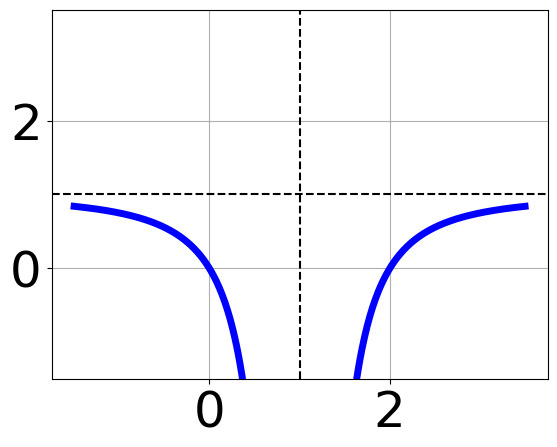
\includegraphics[width=0.5\textwidth]{../Figures/rationalGraphToEquationCopyA.png}
\end{center}


The solution is \( \text{None of the above as it should be } f(x) = \frac{-1}{(x - 1)^2} + 1 \), which is option E.\begin{enumerate}[label=\Alph*.]
\item \( f(x) = \frac{1}{x - 1} + 1 \)

Corresponds to thinking the graph was a shifted version of $\frac{1}{x}$, using the general form $f(x) = \frac{a}{(x-h)^2}+k$, and the opposite leading coefficient.
\item \( f(x) = \frac{-1}{x + 1} + 1 \)

Corresponds to thinking the graph was a shifted version of $\frac{1}{x}$.
\item \( f(x) = \frac{-1}{(x + 1)^2} + 1 \)

The $x$-value of the equation does not match the graph.
\item \( f(x) = \frac{1}{(x - 1)^2} + 1 \)

Corresponds to using the general form $f(x) = \frac{a}{(x-h)^2}+k$ and the opposite leading coefficient.
\item \( \text{None of the above} \)

None of the equation options were the correct equation.
\end{enumerate}

\textbf{General Comment:} Remember that the general form of a basic rational equation is $ f(x) = \frac{a}{(x-h)^n} + k$, where $a$ is the leading coefficient (and in this case, we assume is either $1$ or $-1$), $n$ is the degree (in this case, either $1$ or $2$), and $(h, k)$ is the intersection of the asymptotes.
}
\litem{
Choose the graph of the equation below.
\[ f(x) = \frac{-1}{x - 3} + 3 \]The solution is the graph below, which is option D.
    \begin{center}
        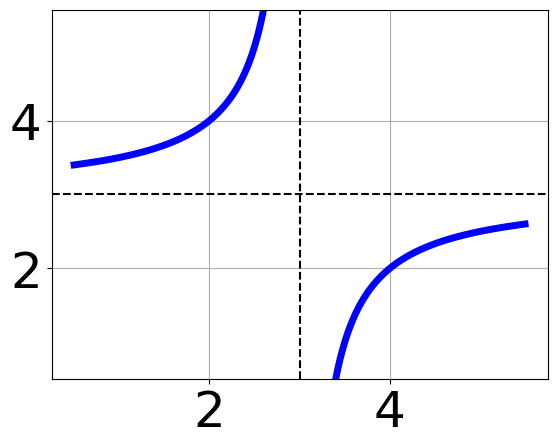
\includegraphics[width=0.3\textwidth]{../Figures/rationalEquationToGraphCopyDA.png}
    \end{center}\begin{enumerate}[label=\Alph*.]
\begin{multicols}{2}
\item 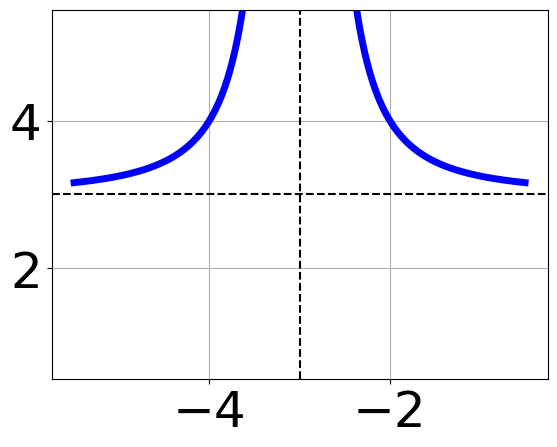
\includegraphics[width = 0.3\textwidth]{../Figures/rationalEquationToGraphCopyAA.png}
\item 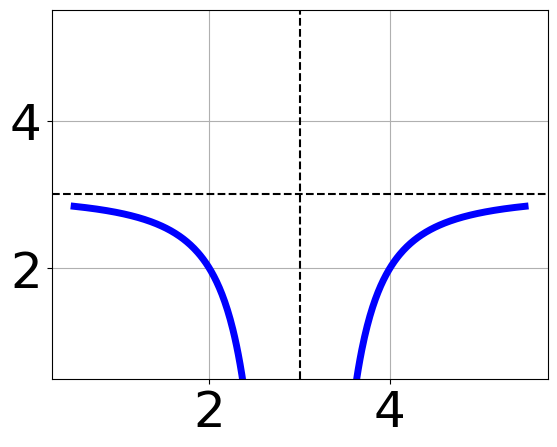
\includegraphics[width = 0.3\textwidth]{../Figures/rationalEquationToGraphCopyBA.png}
\item 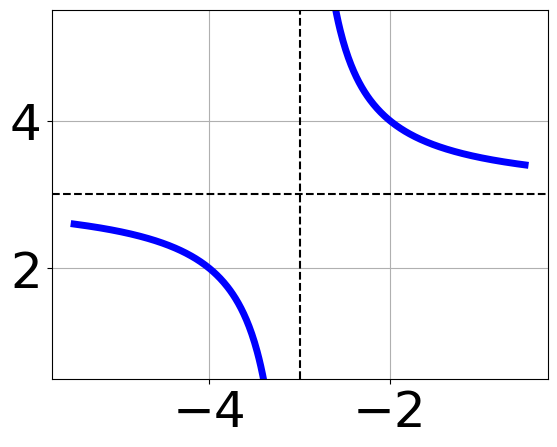
\includegraphics[width = 0.3\textwidth]{../Figures/rationalEquationToGraphCopyCA.png}
\item 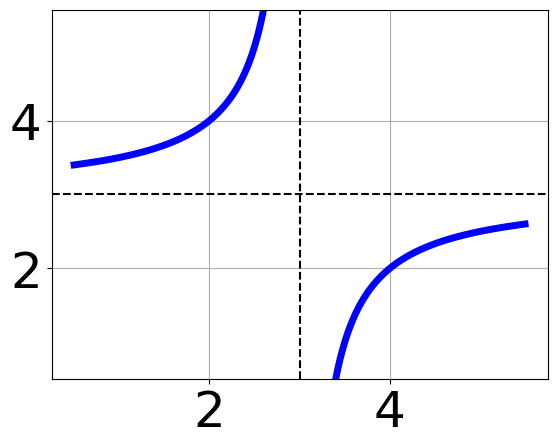
\includegraphics[width = 0.3\textwidth]{../Figures/rationalEquationToGraphCopyDA.png}
\end{multicols}\item None of the above.\end{enumerate}
\textbf{General Comment:} Remember that the general form of a basic rational equation is $ f(x) = \frac{a}{(x-h)^n} + k$, where $a$ is the leading coefficient (and in this case, we assume is either $1$ or $-1$), $n$ is the degree (in this case, either $1$ or $2$), and $(h, k)$ is the intersection of the asymptotes.
}
\litem{
Determine the domain of the function below.
\[ f(x) = \frac{6}{18x^{2} -48 x + 30} \]The solution is \( \text{All Real numbers except } x = 1.000 \text{ and } x = 1.667. \), which is option A.\begin{enumerate}[label=\Alph*.]
\item \( \text{All Real numbers except } x = a \text{ and } x = b, \text{ where } a \in [0.08, 1.26] \text{ and } b \in [1.34, 2.24] \)

All Real numbers except $x = 1.000$ and $x = 1.667$, which is the correct option.
\item \( \text{All Real numbers.} \)

This corresponds to thinking the denominator has complex roots or that rational functions have a domain of all Real numbers.
\item \( \text{All Real numbers except } x = a, \text{ where } a \in [14.2, 15.35] \)

All Real numbers except $x = 15.000$, which corresponds to removing a distractor value from the denominator.
\item \( \text{All Real numbers except } x = a, \text{ where } a \in [0.08, 1.26] \)

All Real numbers except $x = 1.000$, which corresponds to removing only 1 value from the denominator.
\item \( \text{All Real numbers except } x = a \text{ and } x = b, \text{ where } a \in [14.2, 15.35] \text{ and } b \in [35.49, 36.48] \)

All Real numbers except $x = 15.000$ and $x = 36.000$, which corresponds to not factoring the denominator correctly.
\end{enumerate}

\textbf{General Comment:} Recall that dividing by zero is not a real number. Therefore the domain is all real numbers \textbf{except} those that make the denominator 0.
}
\litem{
Solve the rational equation below. Then, choose the interval(s) that the solution(s) belongs to.
\[ \frac{-3}{9x + 7} + 8 = \frac{-8}{-81x -63} \]The solution is \( x = -0.724 \), which is option B.\begin{enumerate}[label=\Alph*.]
\item \( x \in [0.7,0.98] \)

$x = 0.832$, which corresponds to not distributing the factor $9x + 7$ correctly when trying to eliminate the fraction.
\item \( x \in [-1.72,1.28] \)

* $x = -0.724$, which is the correct option.
\item \( x_1 \in [-0.73, -0.57] \text{ and } x_2 \in [0.2,1.3] \)

$x = -0.724 \text{ and } x = 0.832$, which corresponds to getting the correct solution and believing there should be a second solution to the equation.
\item \( \text{All solutions lead to invalid or complex values in the equation.} \)

This corresponds to thinking $x = -0.724$ leads to dividing by zero in the original equation, which it does not.
\item \( x_1 \in [-1.11, -0.79] \text{ and } x_2 \in [-1.2,-0.2] \)

$x = -0.847 \text{ and } x = -0.724$, which corresponds to getting the correct solution and believing there should be a second solution to the equation.
\end{enumerate}

\textbf{General Comment:} Distractors are different based on the number of solutions. Remember that after solving, we need to make sure our solution does not make the original equation divide by zero!
}
\litem{
Choose the graph of the equation below.
\[ f(x) = \frac{-1}{(x + 3)^2} + 2 \]The solution is the graph below, which is option E.
    \begin{center}
        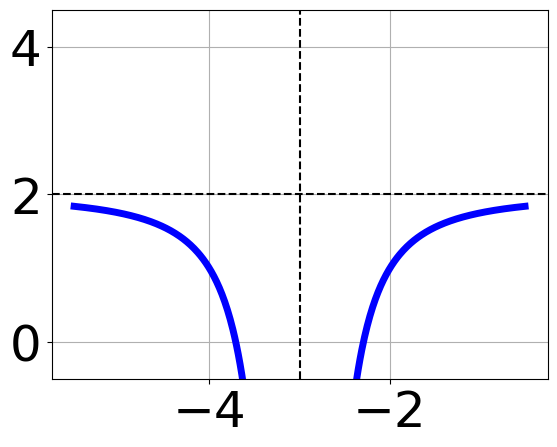
\includegraphics[width=0.3\textwidth]{../Figures/rationalEquationToGraphEA.png}
    \end{center}\begin{enumerate}[label=\Alph*.]
\begin{multicols}{2}
\item 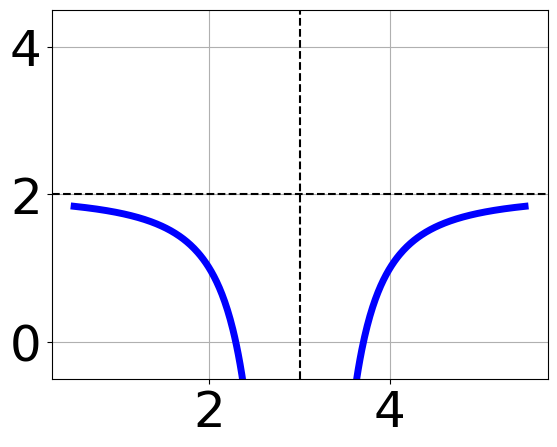
\includegraphics[width = 0.3\textwidth]{../Figures/rationalEquationToGraphAA.png}
\item 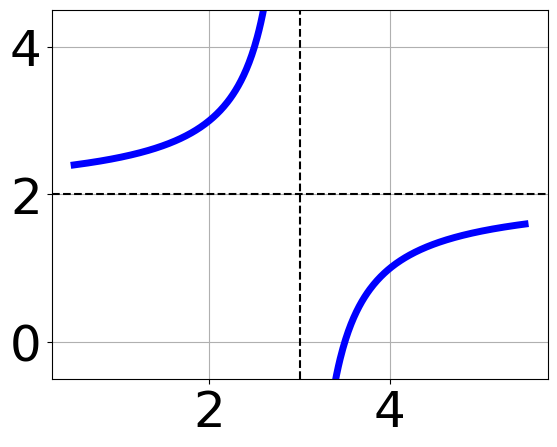
\includegraphics[width = 0.3\textwidth]{../Figures/rationalEquationToGraphBA.png}
\item 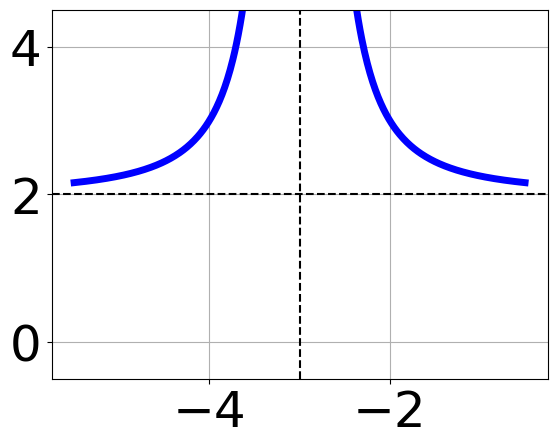
\includegraphics[width = 0.3\textwidth]{../Figures/rationalEquationToGraphCA.png}
\item 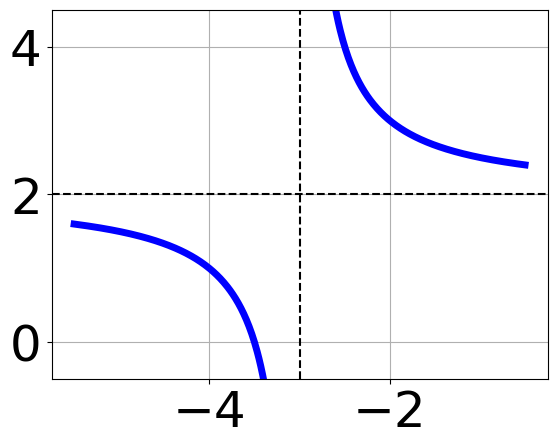
\includegraphics[width = 0.3\textwidth]{../Figures/rationalEquationToGraphDA.png}
\end{multicols}\item None of the above.\end{enumerate}
\textbf{General Comment:} Remember that the general form of a basic rational equation is $ f(x) = \frac{a}{(x-h)^n} + k$, where $a$ is the leading coefficient (and in this case, we assume is either $1$ or $-1$), $n$ is the degree (in this case, either $1$ or $2$), and $(h, k)$ is the intersection of the asymptotes.
}
\litem{
Choose the equation of the function graphed below.

\begin{center}
    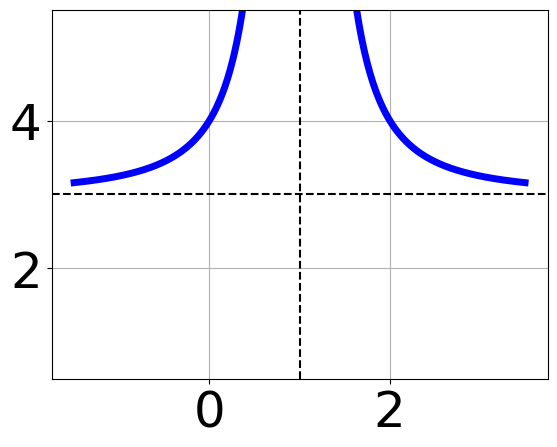
\includegraphics[width=0.5\textwidth]{../Figures/rationalGraphToEquationA.png}
\end{center}


The solution is \( f(x) = \frac{1}{(x - 1)^2} + 3 \), which is option C.\begin{enumerate}[label=\Alph*.]
\item \( f(x) = \frac{-1}{x + 1} + 3 \)

Corresponds to thinking the graph was a shifted version of $\frac{1}{x}$, using the general form $f(x) = \frac{a}{(x+h)^2}+k$, and the opposite leading coefficient.
\item \( f(x) = \frac{-1}{(x + 1)^2} + 3 \)

Corresponds to using the general form $f(x) = \frac{a}{(x+h)^2}+k$ and the opposite leading coefficient.
\item \( f(x) = \frac{1}{(x - 1)^2} + 3 \)

This is the correct option.
\item \( f(x) = \frac{1}{x - 1} + 3 \)

Corresponds to thinking the graph was a shifted version of $\frac{1}{x}$.
\item \( \text{None of the above} \)

This corresponds to believing the vertex of the graph was not correct.
\end{enumerate}

\textbf{General Comment:} Remember that the general form of a basic rational equation is $ f(x) = \frac{a}{(x-h)^n} + k$, where $a$ is the leading coefficient (and in this case, we assume is either $1$ or $-1$), $n$ is the degree (in this case, either $1$ or $2$), and $(h, k)$ is the intersection of the asymptotes.
}
\litem{
Solve the rational equation below. Then, choose the interval(s) that the solution(s) belongs to.
\[ \frac{-4x}{-6x -6} + \frac{-2x^{2}}{-12x^{2} +12 x + 24} = \frac{-3}{2x -4} \]The solution is \( \text{All solutions are invalid or lead to complex values in the equation.} \), which is option B.\begin{enumerate}[label=\Alph*.]
\item \( x_1 \in [-1.52, -0.93] \text{ and } x_2 \in [0,4] \)

$x = -1.000 \text{ and } x = 2.000$, which corresponds to solving $-6x -6 = 0$ and $2x -4 = 0$ and treating them as solutions to the equation.
\item \( \text{All solutions lead to invalid or complex values in the equation.} \)

* The equation leads to solving $-6x^{2} -2 x -18=0$, which leads to complex solutions. This is the correct option.
\item \( x \in [-1.52,-0.93] \)

$x = -1.000$, which corresponds to solving $-6x -6 = 0$ and treating it as a solution to the equation.
\item \( x \in [1.74,3.27] \)

$x = 2.000$, which corresponds to solving $2x -4 = 0$ and treating it as a solution to the equation.
\item \( x_1 \in [1.03, 1.6] \text{ and } x_2 \in [-4.89,-0.89] \)

$x = 1.557 \text{ and } x = -1.891$, which corresponds to making the discriminant from the Quadratic Formula positive to avoid complex solutions.
\end{enumerate}

\textbf{General Comment:} Distractors are different based on the number of solutions. Remember that after solving, we need to make sure our solution does not make the original equation divide by zero!
}
\litem{
Solve the rational equation below. Then, choose the interval(s) that the solution(s) belongs to.
\[ \frac{3x}{5x -2} + \frac{-2x^{2}}{15x^{2} -26 x + 8} = \frac{-4}{3x -4} \]The solution is \( \text{There are two solutions: } x = 0.641 \text{ and } x = -1.784 \), which is option D.\begin{enumerate}[label=\Alph*.]
\item \( x \in [-3.37,0.31] \)


\item \( x \in [0.82,2.75] \)


\item \( x_1 \in [-0.86, 0.67] \text{ and } x_2 \in [0.4,2.4] \)


\item \( x_1 \in [-0.86, 0.67] \text{ and } x_2 \in [-4.78,0.22] \)

* $x = 0.641 \text{ and } x = -1.784$, which is the correct option.
\item \( \text{All solutions lead to invalid or complex values in the equation.} \)


\end{enumerate}

\textbf{General Comment:} Distractors are different based on the number of solutions. Remember that after solving, we need to make sure our solution does not make the original equation divide by zero!
}
\end{enumerate}

\end{document}